\documentclass[11pt,a4paper]{article}
\usepackage[utf8]{inputenc}
\usepackage{amsmath}
\usepackage{amsfonts}
\usepackage{amssymb}
\usepackage{graphicx}

\title{Requirements Analysis Document
		\\FindMeTutor}

\begin{document}
	\maketitle
	\pagenumbering{gobble}
	\newpage
	
	\tableofcontents
	\pagenumbering{roman}
	
	\newpage
	\pagenumbering{arabic}
	\section{Introduction}
		
		\subsection{Purpose of this system}
		The purpose of this system is to provide a safe environment to link students to tutors in the prospect of tutors providing 			students with academic help. 		
		
		%\subsection{Scope}
					
				
		%\section{Stakeholders}
		 
		% \begin{tabular}{| p{10cm}| l |}
		 %	\hline
		 %	\textbf{Stakeholder} & \textbf{Stakeholder Interest} \\ \hline
		 	
		 	%Student  
		 %\end{tabular}
		%Student \\
		%Tutor  \\
		%Administrator \\ 
		%Developer \\
		%Software Design Lecturer \\
	
	\section{Overview}			
	
		\subsection{Functional requirements}
	
		\begin{tabular}{| l | p{10cm}| l |}
			\hline			
			\textbf{Requirement} & \textbf{Functional Requirement} & \textbf{Use Case}
			
			\\ \hline RQ1.1 & The system shall allow a student to register  & UC-CS \\ \hline 
			RQ1.2 & The system shall allow a student to update their account & UC-US \\ \hline  
			RQ1.3 & The system shall allow a student to view their account details  & UC-VS \\ \hline 
			RQ1.4 & The system shall allow a student to mark their account as deleted & UC-DS  \\ \hline 
			RQ2.1 & The system shall allow a tutor to register & UC-CT \\ \hline
			RQ2.2 & The system shall allow a tutor to update their account  & UC-UT \\ \hline
			RQ2.3 & The system shall allow a tutor to view their account details & UC-VT \\ \hline
			RQ2.4 & The system shall allow a tutor to mark their account as deleted & UC-DT \\ \hline  
			
			RQ3.1 & The system shall allow a administrator to update a student account & UC-US \\ \hline  
			RQ3.2 & The system shall allow a administrator to view a student account details  & UC-VS \\ \hline 
			RQ3.3 & The system shall allow a administrator to mark a student as deleted & UC-DS  \\ \hline 
			RQ3.4 & The system shall allow a administrator to update a tutor account  & UC-UT \\ \hline
			RQ3.5 & The system shall allow a administrator to view a tutor account details & UC-VT \\ \hline
			RQ3.6 & The system shall allow a administrator to mark a tutor account as deleted & UC-DT \\ \hline			
			
		\end{tabular}
	
		%\subsection{Non-functional requirements}
		
		
			
	\section{System Models}
		\subsection{	Use cases}
			Create Student		UC-CS
			\\Update Student 	UC-US
			\\View Student      UC-VS
			\\Archive Student	UC-DS
			\\Create Tutor		UC-CT
			\\Update Tutor		UC-UT
			\\View Tutor			UC-VT
			\\Archive Tutor		UC-DT
						
		\subsection{Use case models}
		
		{
		\centering
		
		\begin{tabular}{| l | l| }
			\hline\multicolumn{2}{|c|}{ \textbf{Use Case UC-CS: Create Student}} \\ \hline
			Related Requirements: & RQ1.1 \\ \hline
			Initiating actor: & Student \\ \hline
			Actor goal: & To register on FindMeTutor\\ \hline
			Participating Actors: & External Database System\\ \hline
			Preconditions: & N/A\\ \hline
			Postconditions: & Student is created\\ \hline
			\multicolumn{2}{|l|}{Flow of activities:}\\ \hline
			\multicolumn{2}{|p{15cm}|}{1. Student indicates sign up}\\
			\multicolumn{2}{|p{15cm}|}{2. System displays student sign up form}\\
			\multicolumn{2}{|p{15cm}|}{3. Student enters demographic data, faculty registration details, security answer and password}	\\		
			\multicolumn{2}{|p{15cm}|}{4. System sends demographic data, faculty registration details, security answer and password to external database system}\\
			\multicolumn{2}{|l|}{5. Student is created}	
			\\ \hline		
		\end{tabular}
		
		\begin{tabular}{| l | p{10cm}| }
			\hline\multicolumn{2}{|c|}{ \textbf{Use Case UC-US: Update Student}} \\ \hline
			Related Requirements: & RQ1.2, RQ3.1 \\ \hline
			Initiating actor: & Student or Administrator \\ \hline
			Actor goal: & To update student demographic data, faculty registration details, security answer or password\\ \hline
			Participating Actors: & External Database System\\ \hline
			Preconditions: & Student exists\\ \hline
			Postconditions: & Student is updated\\ \hline
			\multicolumn{2}{|l|}{Flow of activities:}\\ \hline
			\multicolumn{2}{|p{15cm}|}{1. Student/Administrator requests to update Student}\\
			\multicolumn{2}{|p{15cm}|}{2. System displays form to update Student}\\
			\multicolumn{2}{|p{15cm}|}{3. Student/Administrator enters demographic data, faculty registration details or security answer}	\\		
			\multicolumn{2}{|p{15cm}|}{4. System sends demographic data, faculty registration details, security answer or password to external database system}\\
			\multicolumn{2}{|l|}{5. Student is updated}	
			\\ \hline		
		\end{tabular}
		
		\begin{tabular}{| l | l| }
		
			\hline\multicolumn{2}{|c|}{ \textbf{Use Case UC-CT: Create Tutor}} \\ \hline
			Related Requirements: & RQ2.1 \\ \hline
			Initiating actor: & Tutor \\ \hline
			Actor goal: & To register on FindMeTutor\\ \hline
			Participating Actors: & External Database System\\ \hline
			Preconditions: & N/A\\ \hline
			Postconditions: & Tutor is created\\ \hline
			\multicolumn{2}{|l|}{Flow of activities:}\\ \hline
			\multicolumn{2}{|p{15cm}|}{1. Tutor indicates sign up}\\
			\multicolumn{2}{|p{15cm}|}{2. System displays tutor sign up form}\\
			\multicolumn{2}{|p{15cm}|}{3. Tutor enters demographic data, courses tutored, security answer and password}	\\		
			\multicolumn{2}{|p{15cm}|}{4. System sends demographic data, courses tutored details, security answer and to external database system}\\
			\multicolumn{2}{|l|}{5. Tutor is created}	
			\\ \hline		
		\end{tabular}
		
		\begin{tabular}{| l | p{10cm}| }
			\hline\multicolumn{2}{|c|}{ \textbf{Use Case UC-UT: Update Tutor}} \\ \hline
			Related Requirements: & RQ2.2, RQ3.4 \\ \hline
			Initiating actor: & Tutor or Administrator \\ \hline
			Actor goal: & To update Tutor demographic data, courses tutored, security answer or password\\ \hline
			Participating Actors: & External Database System\\ \hline
			Preconditions: Tutor exists\\ \hline
			Postconditions: & Tutor is updated\\ \hline
			\multicolumn{2}{|l|}{Flow of activities:}\\ \hline
			\multicolumn{2}{|p{15cm}|}{1. Tutor/Administrator requests to update Tutor}\\
			\multicolumn{2}{|p{15cm}|}{2. System displays form to update Tutor}\\
			\multicolumn{2}{|p{15cm}|}{3. Tutor/Administrator enters demographic data, faculty registration details or security answer}	\\		
			\multicolumn{2}{|p{15cm}|}{4. System sends demographic data, faculty registration details, security answer or password to external database system}\\
			\multicolumn{2}{|l|}{5. Tutor is updated}	
			\\ \hline		
		\end{tabular}

		}
		
		\subsection{Use case Diagrams}
		
		\begin{figure}[ht!]
		\centering
		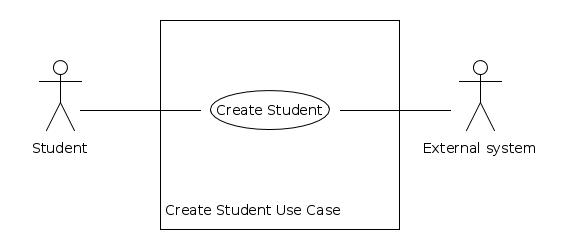
\includegraphics[width=140mm]{/home/shaneel/Documents/FindMeTutor/Use_Cases/Create_Student.jpg}
		Use case diagram: Update Student 		
		
		\end{figure}
		
		\begin{figure}[ht!]
		\centering
		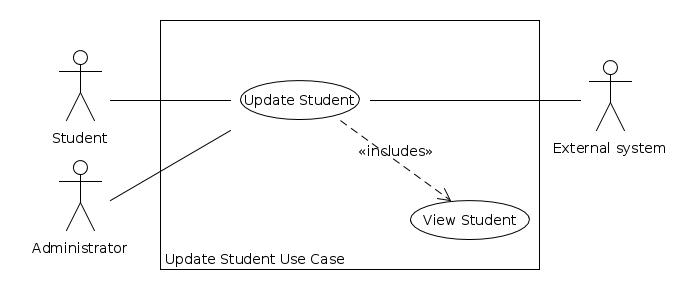
\includegraphics[width=140mm]{/home/shaneel/Documents/FindMeTutor/Use_Cases/Update_Student.jpg}
		Use case diagram: Update Student 
		\end{figure}
		
		\begin{figure}[ht!]
		\centering
		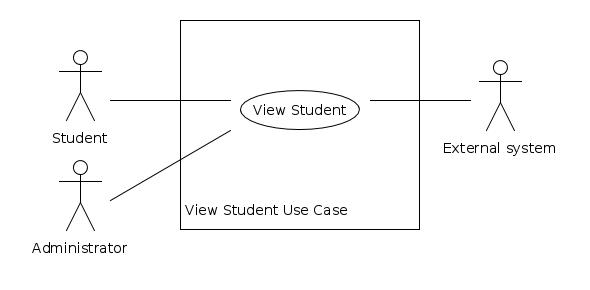
\includegraphics[width=140mm]{/home/shaneel/Documents/FindMeTutor/Use_Cases/View_Student.jpg}
		Use case diagram: View Student 
		\end{figure}
		
		\begin{figure}[ht!]
		\centering
		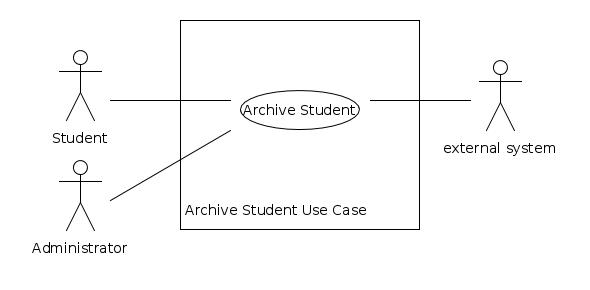
\includegraphics[width=140mm]{/home/shaneel/Documents/FindMeTutor/Use_Cases/Archive_Student.jpg}
		Use case diagram: Archive Student
		\end{figure}
		
		\begin{figure}[ht!]
		\centering
		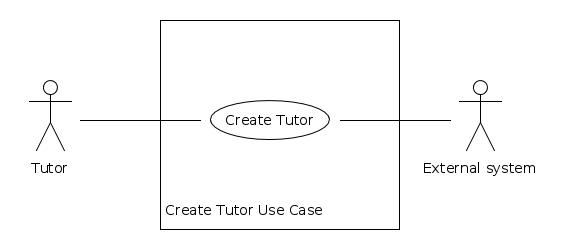
\includegraphics[width=140mm]{/home/shaneel/Documents/FindMeTutor/Use_Cases/Create_Tutor.jpg}
		Use case diagram: Create Tutor
		\end{figure}
		
		\begin{figure}[ht!]
		\centering
		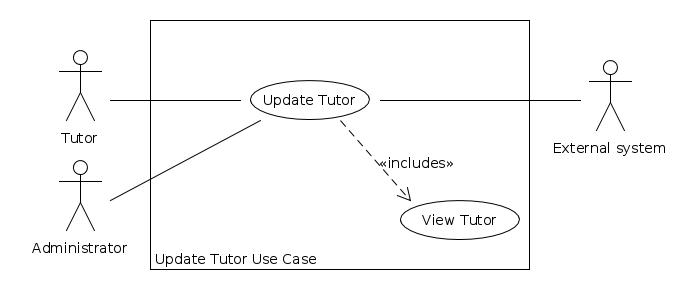
\includegraphics[width=140mm]{/home/shaneel/Documents/FindMeTutor/Use_Cases/Update_Tutor.jpg}
		Use case diagram: Update Tutor
		\end{figure}
		
		\begin{figure}[ht!]
		\centering
		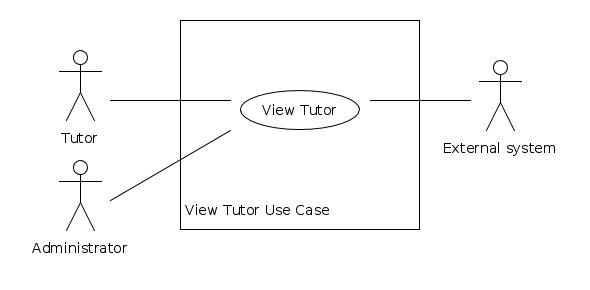
\includegraphics[width=140mm]{/home/shaneel/Documents/FindMeTutor/Use_Cases/View_Tutor.jpg}
		Use case diagram: View Tutor
		\end{figure}
		
		\begin{figure}[ht!]
		\centering
		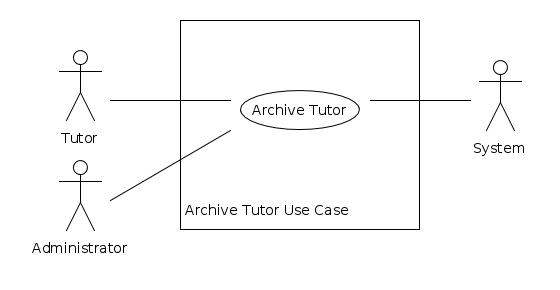
\includegraphics[width=140mm]{/home/shaneel/Documents/FindMeTutor/Use_Cases/Archive_Tutor.jpg}
		Use case diagram: Archive Tutor
		\end{figure}
	
\end{document}
